\documentclass[10pt,hyperref={pdfpagemode=FullScreen},xcolor=dvipsnames,xcolor=table, xcolor=svgnames]{beamer}%,draft
\usepackage[utf8]{inputenc} 
\usepackage[T1]{fontenc} 
\usepackage{lmodern}
\usetheme{Madrid}
%\useinnertheme{rounded}
%\usecolortheme{crane}
\usepackage{pifont}
\usepackage{array}
\usepackage{multirow}
\usepackage{xspace}
\usepackage{tikz}
\usepackage[frenchb]{babel} 

\setbeamersize{text margin right=0.5cm}
\setlength\parindent{0pt}
\newcommand{\latex}{\LaTeX\xspace}

\newcommand{\pat}{\par\vspace{0.5em}}
\newcommand{\koma}{\sffamily KOMA-Script\xspace}
\newcommand{\grille}{
 \begin{tikzpicture}[overlay,remember picture]
  \begin{scope}[shift={(current page.south west)}]
    \draw[gray!50] (0,0) grid[step=2mm] (current page.north east);
    \draw[red!50] (0,0) grid[step=1cm] (current page.north east);
  \end{scope}
\end{tikzpicture}
}

  %%%%%%%%%%%%
 %%%   couleur pour les boites    %%%
 %%%%%%%%%%%%
\definecolor{cadremot}{RGB}{255,0,0}
\definecolor{cadrephrase}{RGB}{0,0,255}
\definecolor{c008000}{RGB}{0,128,0}



\setbeamertemplate{navigation symbols}{} 
\setbeamersize{text margin left =15pt}
\setbeamersize{text margin right =15pt}
\graphicspath{{./images/}}
\DeclareGraphicsExtensions{.png,.jpg,.pdf}
\setlength\fboxsep{0pt}
\begin{document}
\author{Bertrand Masson}
\date{\today} 
\title{\LaTeX{} \& les illustrations}
 \subtitle{ou comment insérer des petits mickeys gnus dans ton texte\\On verra aussi comment triturer du texte}
 \institute{Les fiches de Bébert}
 %%%%%%%%%%%%
 %%%   diapo 1    %%%
 %%%%%%%%


 \begin{frame}{Les fiches de Bébert}
 \titlepage
  \begin{tikzpicture}[overlay,remember picture]
 \draw (6.6,4.8) node{\includegraphics[height=1em,width=4em]{croix}};
 \end{tikzpicture}

 \end{frame}
  %%%%%%%%%%%%
 %%%   diapo 2    %%%
 %%%%%%%%%%%%


  \begin{frame}[fragile]
  \frametitle{Le package graphicx}
%  \begin{block}
Insérer des figures est très simple. Pour cela il faut charger le package \textcolor{blue}{graphicx}, par la commande
{\color{blue}\verb"\usepackage{graphicx}"} dans l'entête de ton fichier source.
\par
  Comme notre but est de fabriquer des fichiers pdf, nous utiliserons uniquement les formats d'images suivants : \textcolor{blue}{.png}, \textcolor{blue}{.jpg} et \textcolor{blue}{.pdf}.\par  La commande pour placer une image \textcolor{blue}{gnu.png} est donc :
\par\bigskip
{\color{blue}\verb"\includegraphics{gnu.png}"}\par
\begin{alertblock}{Attention}
 comme aucun répertoire n'est indiqué \latex va chercher l'image uniquement dans le répertoire courant, c'est à dire celui qui contient le fichier \textcolor{blue}{.tex}
\end{alertblock}
\end{frame}
  %%%%%%%%%%%%
 %%%   diapo 3    %%%
 %%%%%%%%%%%%
 \begin{frame}[fragile]
   \frametitle{Déclarer le chemin du répertoires des images}
  %\begin{block}
Pour faciliter la gestion de mes documents je place mes images dans un répertoire \og images\fg dans le répertoire où se trouve mes fichiers \latex. La commande pour placer une image \textcolor{blue}{gnu.png} est donc :
\begin{exampleblock}{}
\verb"\includegraphics{./images/gnu}"
\end{exampleblock}
Tu peux définir le chemin du répertoire ou \latex doit aller chercher les images par :
{\color{blue}\verb"\graphicspath{{./images/}}"}. L'expression {\color{blue}\verb"./images/"}, signifie dans le répertoire \og images\fg du répertoire courant. Tu places cette commande dans le préambule de ton source (avant {\color{blue}\verb"\begin{document}"}).\par
Si tu as trié tes illustrations dans différents répertoires en fonction de leur nature (schémas, photos, courbes), il te faudra utiliser la commande 
\begin{exampleblock}{}
\verb"\graphicspath{{./dossier1/}{./dossier2/}...{./dossierN/}}"
\end{exampleblock}
\begin{alertblock}{Attention}
Même si tu ne déclares qu'un seul répertoire il doit être entouré de \textcolor{blue}{\{\}}, et n'oublie pas la barre de fraction (\textcolor{blue}{/}) finale.
\end{alertblock}
\end{frame}
  %%%%%%%%%%%%
 %%%   diapo 4    %%%
 %%%%%%%%%%%%
 \begin{frame}[fragile]
   \frametitle{Déclarer les extensions des images}
%  \begin{block}
Tu peux t'abstenir de préciser l'extension si tu as mis dans le préambule de ton document la commande : 
\begin{exampleblock}{}
\verb"\DeclareGraphicsExtensions{.png,.jpg,.pdf}"
\end{exampleblock}
 Dans l'exemple ci-dessus, \latex  va d'abord chercher l'existence d'un fichier en  \textcolor{blue}{.png}, s'il ne trouve pas, un fichier en  \textcolor{blue}{.jpg} et enfin en \textcolor{blue}{.pdf}.\par Tu peux bien évidemment changer l'ordre.
 \par
 Dans les exemples qui suivent on va considérer que j'ai déclaré le chemin et les extentions.
%\end{block}
\end{frame}
  %%%%%%%%%%%%
 %%%   diapo 4    %%%
 %%%%%%%%%%%%
 \begin{frame}[fragile]
   \frametitle{Notre première image}
 
On va placer notre première image dans un document \latex. Voici le code :
\par
\begin{exampleblock}{}
\begin{verbatim}
Un logo gnu \includegraphics{gnu} et
un logo debian \includegraphics{debian}.
\end{verbatim}
\end{exampleblock}
et voici le résultat :
\begin{block}{}
Un logo gnu \includegraphics[scale=0.4]{gnu}\, et un logo debian \includegraphics[scale=0.4]{debian}.
\end{block}
Nos logos sont un peu grands. Sans précision {\color{blue}\verb"\includegraphics"} affiche le dessin dans sa taille réelle soit pour le logo gnu 125x50 pixels.
\par
Pour remédier à celà {\color{blue}\verb"\includegraphics"} accepte des options du type \textcolor{blue}{option=valeur}, séparées par des virgules.
\begin{exampleblock}{}
\verb"\includegraphics[option1=valeur1,option2=valeur2]{gnu}"
\end{exampleblock}
\end{frame}
  %%%%%%%%%%%%
 %%%   diapo 5    %%%
 %%%%%%%%%%%%
 \begin{frame}[fragile]
   \frametitle{Dimensionner les images}
Comme on va manipuler des longueurs, je te conseille, si ce n'est déjà fait, la lecture de la fiche \og\latex et les longueurs\fg.\par
Tu peux commencer par modifier l'échelle de ton image par l'option {\color{blue}\verb!scale!}. Des valeurs supérieur à 1 augmentent la taille de l'image  ({\color{blue}\verb!scale=2!} double la taille), des valeurs comprises entre 0 et 1 diminuent la taille ({\color{blue}\verb!scale=0.5!} divise par 2 les dimensions).
\begin{exampleblock}{}
\begin{verbatim}
Un logo gnu \includegraphics[scale=0.3]{gnu} et
un logo debian \includegraphics[scale=0.5]{debian}.
\end{verbatim}
\end{exampleblock}
\begin{block}{}
Un logo gnu \includegraphics[scale=0.12]{gnu}\, et un logo debian \includegraphics[scale=0.25]{debian}.
\end{block}
\end{frame}
  %%%%%%%%%%%%
 %%%   diapo 6    %%%
 %%%%%%%%%%%%
 \begin{frame}[fragile]
   \frametitle{Dimensionner les images}
Tu peux également donner directement les dimensions souhaitées pour l'image. L'option {\color{blue}\verb!width!} règle la largeur de l'image et {\color{blue}\verb!height!} sa hauteur. Comme le but ici est d'intégrer notre image dans du texte, j'utilise l'em qui équivaut à la taille de la lettre m. Si tu ne donnes qu'une seule dimension les proportions de l'image seront conservées.
\begin{exampleblock}{}
\begin{verbatim}
Un logo gnu \includegraphics[width=2em]{gnu} et
un logo debian \includegraphics[height=2.5em]{debian}.
\end{verbatim}
\end{exampleblock}
\begin{block}{}
Un logo gnu \includegraphics[width=2em]{gnu}\, et un logo debian \includegraphics[height=2.5em]{debian}.
\end{block}
\end{frame}
  %%%%%%%%%%%%
 %%%   diapo 7    %%%
 %%%%%%%%%%%%
 \begin{frame}[fragile]
   \frametitle{Dimensionner les images}
Tu n'es pas obligé de conserver les proportions :
\begin{exampleblock}{}
\begin{verbatim}
Un logo gnu \includegraphics[width=6em,height=1em]{gnu} et
un logo debian \includegraphics[width=0.5em,height=3em]{debian}.
\end{verbatim}
\end{exampleblock}
\begin{block}{}
Un logo gnu \includegraphics[width=6em,height=1em]{gnu}\, et un logo debian \includegraphics[width=0.5em,height=3em]{debian}.
\end{block}
L'option {\color{blue}\verb!keepaspectratio!}, qui est un booléen prenant les valeurs {\color{blue}\verb!true!} et  {\color{blue}\verb!false!} permet de ne pas déformer l'image, et dimensionne l'image de telle sorte que les proportions soit respectées et que ni la largeur ni la hauteur ne dépassent les valeurs données à {\color{blue}\verb!width!} et {\color{blue}\verb!height!}
\begin{exampleblock}{}
\footnotesize
\begin{verbatim}
Un logo gnu \includegraphics[width=6em,height=1em,keepaspectratio=true]{gnu} et
un logo debian
\includegraphics[width=0.5em,height=3em,keepaspectratio=true]{debian}.
\end{verbatim}
\end{exampleblock}
\begin{block}{}
Un logo gnu \includegraphics[width=6em,height=1em,keepaspectratio=true]{gnu}\, et un logo debian \includegraphics[width=0.5em,height=3em,keepaspectratio=true]{debian}.
\end{block}
\end{frame}
  %%%%%%%%%%%%
 %%%   diapo 8    %%%
 %%%%%%%%%%%%
 \begin{frame}[fragile]
   \frametitle{Rotation des images}
Pour faire tourner l'image on utilise l'option {\color{blue}\verb!angle=nombreEnDegrés!} :
\begin{exampleblock}{}
\begin{verbatim}
Un logo gnu \includegraphics[width=3em,angle=45]{gnu} et
un autre logo gnu \includegraphics[width=3em,angle=-45]{gnu}.
\end{verbatim}
\end{exampleblock}
\begin{block}{}
Un logo gnu \includegraphics[width=3em,angle=45]{gnu} et
un autre logo gnu \includegraphics[width=3em,angle=-45]{gnu}.
\end{block}
Tu peux préciser l'origine de la rotation. Auparavant on va aborder la notion de boite sous \latex.
\end{frame}
%%%%%%%%%%%%
 %%%   diapo 9    %%%
 %%%%%%%%%%%
 \begin{frame}[fragile]
   \frametitle{\latex et les boites}
\onslide<1-> 
\begin{center}
{\fontsize{45}{45}\selectfont Un petit} \includegraphics[scale=0.25]{gnuOrange}\, {\fontsize{45}{45}\selectfont gnu}
\end{center}


\onslide<1->Pour \latex tout est boite. \latex ne compose pas des mots avec des lettres mais manipule des boites qui contiennent des objets. Un peu comme les ouvriers typographes et leurs caractères en plomb.\par
\onslide<2->
\begin{tikzpicture}[overlay,remember picture]
	\begin{scope}[shift={(current page.south west)}] 
    		\draw (1.15,6.8) rectangle (2.15,7.9);
    		\draw (2.15,6.8) rectangle (2.9,7.5);
    		\draw (2.9,6.8) rectangle (3.47,7.5);
    		\draw (3.47,6.5) rectangle (4.2,7.5);
    		\draw (4.2,6.8) rectangle (4.9,7.5);
    		\draw (4.9,6.8) rectangle (5.45,7.7);
    		\draw (5.45,6.8) rectangle (5.75,7.85);
    		\draw (5.75,6.8) rectangle (6.3,7.7);
    		\draw (6.3,6.8) rectangle (9.3,7.9);
    		\draw (9.3,6.5) rectangle (10.1,7.5);
    		\draw (10.1,6.8) rectangle (10.9,7.5);
    		\draw (10.9,6.8) rectangle (11.6,7.5);
    	 \end{scope}   
\end{tikzpicture}
\onslide<2->
On a donc des boites qui contiennent des lettres. 
\onslide<3-4,6-7>
\begin{tikzpicture}[overlay,remember picture]
	\begin{scope}[shift={(current page.south west)},draw=red] 
    		\draw (1.15,6.8) rectangle (2.9,7.9);
    		\draw (3.47,6.25) rectangle (6.3,7.85);
    		\draw (9.3,6.25) rectangle (11.6,7.5);    	
    	 \end{scope}   
\end{tikzpicture}
\onslide<3->Puis des boites de mots contenant des boites de lettres
\onslide<4,7>
\begin{tikzpicture}[overlay,remember picture]
	\begin{scope}[shift={(current page.south west)},draw=blue] 
    		\draw (1.15,6.25) rectangle (11.6,7.9);  	
    	 \end{scope}   
\end{tikzpicture}
\onslide<4->et enfin des boites de phrases contenant des boites de mots. Le logo gnu est aussi mis en boite.\par
\onslide<5->
\begin{tikzpicture}[overlay,remember picture]
	\begin{scope}[shift={(current page.south west)}] 
    		\draw (1.15,6.8) circle (2pt);
    		\draw (2.15,6.8) circle (2pt);
    		\draw (2.9,6.8) circle (2pt);
    		\draw (3.47,6.8) circle (2pt);
    		\draw (4.2,6.8) circle (2pt);
    		\draw (4.9,6.8) circle (2pt);
    		\draw (5.45,6.8) circle (2pt);
    		\draw (5.75,6.8) circle (2pt);
    		\draw (6.3,6.8) circle (2pt);
    		\draw (9.3,6.8) circle (2pt);
    		\draw (10.1,6.8) circle (2pt);
    		\draw (10.9,6.8) circle (2pt);
    	 \end{scope}   
\end{tikzpicture}
\onslide<5->Chaque boite à une origine.\par
\onslide<6-7>\begin{tikzpicture}[overlay,remember picture]
	\begin{scope}[shift={(current page.south west)},draw=red] 
    		\draw (1.15,6.8) circle (2pt);
       		\draw (2.9,6.8) circle (2pt);
    		\draw (3.47,6.8) circle (2pt);
    		\draw (6.3,6.8) circle (2pt);  	
    	 \end{scope}   
\end{tikzpicture}
\onslide<7>
\begin{tikzpicture}[overlay,remember picture]
	\begin{scope}[shift={(current page.south west)},draw=blue] 
    		\draw (1.15,6.8) circle (2pt); 
    	 \end{scope}   
\end{tikzpicture}
\onslide<8>
\begin{tikzpicture}[overlay,remember picture]
	\begin{scope}[shift={(current page.south west)},draw=green,thick] 
    		\draw (0,6.8) -- (12.8,6.8); 
    	 \end{scope}   
\end{tikzpicture}
\onslide<8->\noindent
\latex place cet origine sur une ligne appelée ligne de base. Tu peux remarquer que cette origine n'est pas toujours au coin en bas à gauche (lettres p et g).\par
\onslide<9->Les boites \latex ont trois dimensions : une largeur, une hauteur et une profondeur qui correspond à ce qui se trouve sous la ligne de base. Dans notre exemple, toutes les boites lettres ont une profondeur nulle à l'exception du p et du g.
\end{frame}

  %%%%%%%%%%%%
 %%%   diapo 10    %%%
 %%%%%%%%%%%%
 \begin{frame}[fragile]
   \frametitle{\latex et les boites}
 En reprenant notre lettre g, voici les différentes longueurs associées à une boite : 
\par
\vspace{1cm}
\begin{center}
{\fontsize{200}{72}\selectfont g}
\end{center}
\begin{tikzpicture}[overlay,remember picture]
	\begin{scope}[shift={(current page.south west)}] 
    		\draw[draw=green,ultra thick] (0,3) -- (12.8,3); 
    		\draw (1.5,3) node[above]{ligne de base};
    		\draw (4.75,1.6) rectangle (8.08,6.17);
    		\draw [<->](4.7,1) --  (8.08,1) node[fill=white,midway]{width} node[midway,below]{(largeur)};
    		\draw [<->](8.5,3) --  (8.5,6.17)  node[fill=white,midway,sloped]{height} node[midway,sloped,below]{(hauteur)};
    		\draw [<->](8.5,1.6) --  (8.5,3); 
    		\draw [<->](11,1.6) --  (11,6.17) node[fill=white,midway,sloped]{totalheight} node[midway,sloped,below]{(hauteur totales)};
    		\draw (9.5,2.3) node {depth};
    		\draw (9.5,2) node {(profondeur)};
    		\draw[draw=red,semithick] (4.75,3) circle (4pt);
    		\node (o) at (4.75,3) {};
    		\node (b) at (2,5) {origine};
    		\draw [->] (b) --(o);
    	 \end{scope}   
\end{tikzpicture}
\end{frame}
  %%%%%%%%%%%%
 %%%   diapo 10    %%%
 %%%%%%%%%%%%
 \begin{frame}[fragile]
   \frametitle{\latex et les boites}
En plus des options {\color{blue}\verb!width!} et {\color{blue}\verb!heigth!} que l'on a vu précédement, {\color{blue}\verb!\includegraphics!} reconnait également {\color{blue}\verb!totalheigth!} et {\color{blue}\verb!depth!}.
\end{frame}

  %%%%%%%%%%%%
 %%%   diapo 11    %%%
 %%%%%%%%%%%%
 \begin{frame}[fragile]
   \frametitle{Rotation des images}
Revenons à notre rotation :
\begin{block}{}
Un logo gnu \includegraphics[width=3em,angle=45]{gnu} et
un autre logo gnu \includegraphics[width=3em,angle=-45]{gnu}.
\end{block}
Comme tu peux le constater par défaut la rotation s'effectue par rapport à l'origine de la boite sur la ligne de base. On peut modifier le centre de rotation à l'aide de l'option {\color{blue}\verb!origin=valeur!}. Les valeurs possibles pour  {\color{blue}\verb!origin!} sont : c (center), b (bottom), t (top), r (right), l (left), B (ligne de base) et des combinaisons de ces valeurs, comme cr ou lt. Tu trouveras un schéma explicatif page suivante. Voici un exemple avec {\color{blue}\verb!origin=c!} pour le premier gnu et  {\color{blue}\verb!origin=rt!} pour le second.
\begin{block}{}
Un logo gnu \includegraphics[width=3em,angle=45,origin=c]{gnu} et
un autre logo gnu \includegraphics[width=3em,angle=-45,origin=rt]{gnu}.
\end{block}
\end{frame}
  %%%%%%%%%%%%
 %%%   diapo 11    %%%
 %%%%%%%%%%%%
 \begin{frame}[fragile]
   \frametitle{Rotation des images}
\begin{center}
\begin{tikzpicture}
\draw[draw=green,ultra thick](-2,1.5)--(8,1.5);
\draw (0,0) rectangle (6,4);
\draw (0,0) node [anchor=north east] {[lb]};
\draw (0,4) node [anchor=south east] {[lt]};
\draw (6,0) node [anchor=north west] {[rb]};
\draw (6,4) node [anchor=south west] {[rt]};
\draw (3,4) node [above] {[ct] ou [t]};
\draw (3,0) node [below] {[cb] ou [b]};
\draw (3,2) node  {[c]};
\draw[draw=red,semithick] (0,1.5) circle (4pt);
    		\node (o) at (0,1.5) {};
    		\node (b) at (-2,3) {origine};
    		\draw [->] (b) --(o);
\draw (0,1.5) node [anchor=north east] {[lB]};
\draw (3,1.5) node [below] {[cB] ou [B]};
\draw (6,1.5) node [anchor=north west] {[rB]};
\draw (-3,1.7) node[above,right]{ligne de base};
\end{tikzpicture}
\end{center}

\end{frame}
  %%%%%%%%%%%%
 %%%   diapo  12   %%%
 %%%%%%%%%%%%
 \begin{frame}[fragile]
   \frametitle{Rotation des images}
 \alert{Attention} l'ordre des options est importante : 
\begin{exampleblock}{}
\begin{verbatim}
\includegraphics[height=3.5em,angle=45,origin=c]{gnu} 
\includegraphics[angle=45,height=3.5em,origin=c]{gnu}
\end{verbatim}
\end{exampleblock}
\vspace{1cm}
\hspace{2cm}\includegraphics[height=3.5em,angle=45,origin=c]{gnu} \hfill \includegraphics[origin=c,angle=45,height=3.5em]{gnu}\hspace{2cm}
\par\vspace{0.5cm}
\latex exécute les commandes de gauche à droite. Dans le premier cas il va d'abord dimensionner l'image puis effectuer une rotation. Dans le second cas il va effectuer une rotation puis appliquer le dimensionement sur l'objet tourné. Je te rapelle que {\color{blue}\verb!height!} conserne que ce qui est audessus de la ligne de base.

\begin{tikzpicture}[overlay,remember picture]
	\begin{scope}[shift={(current page.south west)}] 
    		\draw[draw=green,ultra thick] (0,3.4) -- (12.8,3.4); 
    		\draw[xshift=3cm,rotate=45] (2.09,1.52) rectangle (5.18,2.8);
    		\draw[<->,xshift=3cm,rotate=45] (5.3,1.52)--(5.3,2.8) ;
    		\draw[xshift=3cm,rotate=45] (5.8,2.16) node{3.5em};
    		\draw (8.7,3) rectangle (10.25,4.5);
    		\draw[<->](10.4,3.4) -- (10.4,4.5);
    		\draw (11,3.95) node{3.5em};
    	 \end{scope}   
\end{tikzpicture}
\end{frame}
  %%%%%%%%%%%%
 %%%   diapo 8    %%%
 %%%%%%%%%%%%
 \begin{frame}[fragile]
   \frametitle{Inclure des fichiers pdf}
Inclusion de fichier pdf se fait de la même façon que n'importe quelle image. Tu as une option supplémentaire  {\color{blue}\verb!page=!} qui permet de choisir la page importée (par défaut c'est la première). Voici deux exemples :
\begin{exampleblock}{}
\begin{verbatim}
\includegraphics[scale=0.25]{illustration}
\includegraphics[scale=0.25,page=2,angle=45]{illustration}
\end{verbatim}
\end{exampleblock}
\hspace{1cm}\includegraphics[scale=0.25]{illustration2}\hfill \includegraphics[scale=0.25,page=2,angle=45]{illustration2}\hspace{1cm}
\end{frame}
  %%%%%%%%%%%%
 %%%   diapo 8    %%%
 %%%%%%%%%%%%
 \begin{frame}[fragile]
   \frametitle{Inclure des fichiers pdf}
Il est possible d'afficher qu'une partie de la page à l'aide des options {\color{blue}\verb!trim=a b c d!} et {\color{blue}\verb!clip!}. Les quatre valeurs prisent par {\color{blue}\verb!trim!} corespondent à la quantité d'espace à rogner à gauche pour a, en bas pour b, à droite pour c et en haut pour d. L'unité utilisée est le \og inch \fg, 1in = 72pt. {\color{blue}\verb!clip!} découpe l'image aux dimensions définies par {\color{blue}\verb!trim!}. Je trouve que cette option n'est pas très facile à utiliser et je l'utilise de manière empirique, car il n'est pas facile de voir à quoi correspond 1in sur une page en pdf. Voici un exemple ou je centre grossièrement l'image sur le logo gnu de la page 5 du pdf que tu es en train de lire. 
\begin{exampleblock}{}\footnotesize
\begin{verbatim}
\includegraphics[scale=0.5,trim=60 60 150 80,clip,page=5]{illustration}
\end{verbatim}
\end{exampleblock}
\begin{center}
\includegraphics[scale=0.5,trim=60 60 150 80,clip,page=5]{illustration2}
\end{center}
Tu peux utiliser cette technique avec n'importe quelle image, mais je trouve plus pratique de préparer convenablement les images avec gimp. 
\end{frame}
  %%%%%%%%%%%%
 %%%   diapo 8    %%%
 %%%%%%%%%%%%
 \begin{frame}[fragile]
   \frametitle{manipuler du texte}
En plus de la commande {\color{blue}\verb!\includegraphics!} le package {\color{blue}\verb!graphicx!} possède d'autres commandes qui permettent de manipuler du texte (ou tout autre objet \latex). {\color{blue}\verb!\scalebox!} et {\color{blue}\verb!\resizebox!} qui permettent d'agrandir ou de rétrécir un objet, {\color{blue}\verb!\reflectbox!}, crée un miroir de l'objet et {\color{blue}\verb!\rotatebox!} qui opère des rotations.
\end{frame}


  %%%%%%%%%%%%
 %%%   diapo 8    %%%
 %%%%%%%%%%%%
 \begin{frame}[fragile]
   \frametitle{Manipuler du texte : scalebox}
{\color{blue}\verb!\scalebox!} fonctionne comme l'option {\color{blue}\verb!\scale!} de {\color{blue}\verb!\includegraphics!}, elle agit sur l'échelle d'un objet :
{\color{blue}\verb!\scalebox{échelleLargeur}[échelleHauteur]{objetLaTeX}!}\par
\begin{exampleblock}{}
\begin{verbatim}
Un texte normal, \scalebox{3}{un très grand texte} et
\scalebox{0.3}{un tout petit texte.}
\end{verbatim}
\end{exampleblock}
\begin{block}{}
Un texte normal, \scalebox{3}[2]{un très grand texte} et \scalebox{0.3}{un tout petit texte.}
\end{block}
{\color{blue}\verb![échelleHauteur]!} est entre [] et est donc optionelle. Si tu ne la précises pas l'objet sera déformé en conservant ses proportions.
\begin{exampleblock}{}
\begin{verbatim}
\scalebox{1}[4]{Un texte déformé}
\end{verbatim}
\end{exampleblock}
\begin{block}{}
\scalebox{1}[4]{Un texte déformé}
\end{block}
\end{frame}

  %%%%%%%%%%%%
 %%%   diapo 8    %%%
 %%%%%%%%%%%%
 \begin{frame}[fragile]
   \frametitle{Manipuler du texte : reflectbox}
{\color{blue}\verb!\reflectbox!} et un raccourci pour 
{\color{blue}\verb!\scalebox{-1}[1]{objetLaTeX}!} qui permet d'écrir en miroir.\par
\begin{exampleblock}{}
\begin{verbatim}
Un texte normal, \reflectbox{un texte miroir}
\end{verbatim}
\end{exampleblock}
\begin{block}{}
Un texte normal, \reflectbox{un texte miroir}
\end{block}
Tu peux t'amuser en variant les facteurs d'échelle :
\begin{exampleblock}{}
\begin{verbatim}
\scalebox{1}[-2]{Un texte miroir} \reflectbox{un texte miroir}
\end{verbatim}
\end{exampleblock}
\begin{block}{}
\scalebox{1}[-2]{Un texte miroir} \reflectbox{un texte miroir}
\end{block}
L'utilisation d'une {\color{blue}\verb!\makebox!} de largeur nulle est intéressante,  \alert{attention} le deuxième argument de la {\color{blue}\verb!\makebox!} est la lettre L minuscule :
\begin{exampleblock}{}\footnotesize
\begin{verbatim}
\makebox[0mm][l]{Un texte miroir}\scalebox{1}[-1]{Un texte miroir}
\end{verbatim}
\end{exampleblock}
\begin{block}{}
\makebox[0mm][l]{Un texte miroir}\scalebox{1}[-1]{Un texte miroir}
\end{block}
\end{frame}
  %%%%%%%%%%%%
 %%%   diapo 8    %%%
 %%%%%%%%%%%%
 \begin{frame}[fragile]
   \frametitle{Manipuler du texte : resizebox}
Tu peux préciser les dimensions verticales et horizontale avec la commande {\color{blue}\verb!\resizebox{dimension horizontale}{dimension verticale}!}. Tu peux conserver les proportions en n'indiquant qu'une seule dimension l'autre étant remplacée par un \og ! \fg
\begin{exampleblock}{}
\begin{verbatim}
\resizebox{!}{1cm}{Un texte} et 
\resizebox{1cm}{10mm}{un autre texte}
\end{verbatim}
\end{exampleblock}
\begin{block}{}
\resizebox{!}{1cm}{Un texte} et \resizebox{1cm}{10mm}{un autre texte}
\end{block}
Tu peux mettre dans ces boites ({\color{blue}\verb!\reflectbox!},{\color{blue}\verb!\scalebox!}, {\color{blue}\verb!\resizebox!} et {\color{blue}\verb!\rotatebox!}) n'importe quel matériel \latex, comme des listes, d'autres boites, des tableaux\dots
Tu trouveras page suivante un exemple avec un tableau.
\end{frame}
  %%%%%%%%%%%%
 %%%   diapo 8    %%%
 %%%%%%%%%%%%
 \begin{frame}[fragile]
   \frametitle{Manipuler du texte : resizebox}
Le premier tableau est normal, le second est créé par la commande suivante :
\begin{exampleblock}{}
\begin{verbatim}
\resizebox{4cm}{3cm}{%
\begin{tabular}{|c|c|c|}
\hline
Banane&Poire&Radis\\\hline
Choucroute&Andouille&Fraise\\\hline
Pou&Hibou&Genou\\\hline
\end{tabular}}  
\end{verbatim}
\end{exampleblock}
\begin{block}{} \hspace{1cm}
\begin{tabular}{|c|c|c|}
\hline
Banane&Poire&Radis\\\hline
Choucroute&Andouille&Fraise\\\hline
Pou&Hibou&Genou\\\hline
\end{tabular}\hfill
\resizebox{3cm}{2cm}{%
\begin{tabular}{|c|c|c|}
\hline
Banane&Poire&Radis\\\hline
Choucroute&Andouille&Fraise\\\hline
Pou&Hibou&Genou\\\hline
\end{tabular}} \hspace{1cm}
\end{block}
\end{frame}

 %%%%%%%%%%%%
 %%%   diapo 8    %%%
 %%%%%%%%%%%%
 \begin{frame}[fragile]
   \frametitle{Manipuler du texte : rotatebox}
Tu effectues la rotation de texte avec :
{\color{blue}\verb!\rotatebox[option=valeur]{angle en degrés}{le texte}!}\par
Option peut être {\color{blue}\verb!origin!} que l'on a vue précédemment et qui prend les mêmes valeurs et {\color{blue}\verb!x=dimension!} et {\color{blue}\verb!y=dimension!} qui permettent de donner les coordonnées du point de rotation.
\begin{exampleblock}{}\footnotesize
\begin{verbatim}
Un \rotatebox{45}{texte} et un autre \rotatebox[c]{45}{texte}
et un troisième \rotatebox{-45}{texte} 
\end{verbatim}
\end{exampleblock}
\begin{block}{}
Un \rotatebox{45}{texte} et un autre \rotatebox[c]{45}{texte} et un troisième \rotatebox{-45}{texte} 
\end{block}
\begin{exampleblock}{}\footnotesize
\begin{verbatim}
Un \rotatebox[x=10mm, y=0mm]{45}{texte} et un autre
\rotatebox[x=1mm, y=15mm]{45}{texte}
\end{verbatim}
\end{exampleblock}
\begin{block}{}
Un \rotatebox[x=5mm, y=0mm]{45}{texte} et un autre \rotatebox[x=1mm, y=10mm]{45}{texte}
\end{block}
\end{frame}
 %%%%%%%%%%%%
 %%%   diapo 8    %%%
 %%%%%%%%%%%%
 \begin{frame}
   \frametitle{Conclusion}
On vient de voir les commandes de bases pour placer des images et manipuler des objets. Une prochaine fiche montrera comment placer harmonieusement tes figures dans ton texte (la notion de flottants), ajouter des légendes, une table des figures\dots
\end{frame}
\end{document}
 